% REDI Architecture Diagram
% For paper: "REDI: Automated Data Readiness for Scientific AI"
%
% Compile with: pdflatex redi_architecture.tex
% or include in your main paper document

\documentclass[tikz,border=10pt]{standalone}
\usepackage{tikz}
\usetikzlibrary{shapes.geometric, arrows.meta, positioning, fit, backgrounds, calc, shadows.blur, decorations.pathreplacing}

% Color scheme - scientific/professional
\definecolor{rediblue}{RGB}{41, 98, 255}
\definecolor{redipurple}{RGB}{103, 58, 183}
\definecolor{redigreen}{RGB}{0, 150, 136}
\definecolor{rediorange}{RGB}{255, 152, 0}
\definecolor{redired}{RGB}{244, 67, 54}
\definecolor{redigray}{RGB}{96, 125, 139}
\definecolor{lightbg}{RGB}{245, 247, 250}
\definecolor{darktext}{RGB}{33, 37, 41}

\begin{document}
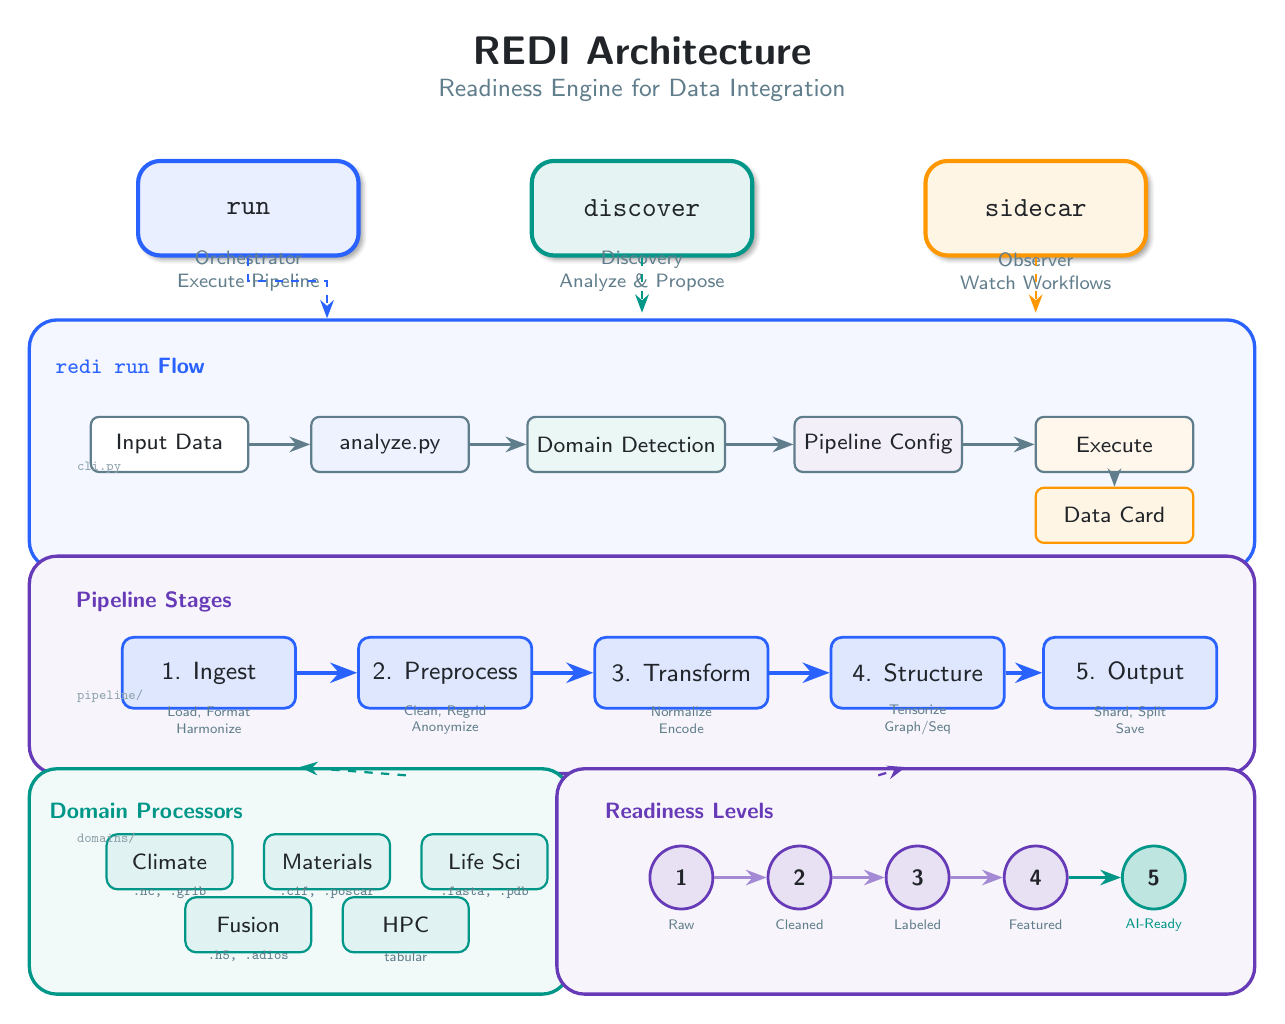
\begin{tikzpicture}[
    % Node styles
    mode/.style={
        rectangle, rounded corners=8pt, minimum width=2.8cm, minimum height=1.2cm,
        draw=#1, line width=1.5pt, fill=#1!10, font=\bfseries\sffamily,
        text=darktext, blur shadow={shadow blur steps=5, shadow xshift=0.5mm, shadow yshift=-0.5mm}
    },
    stage/.style={
        rectangle, rounded corners=4pt, minimum width=2.2cm, minimum height=0.9cm,
        draw=rediblue, line width=1pt, fill=rediblue!15, font=\sffamily\small,
        text=darktext
    },
    domainnode/.style={
        rectangle, rounded corners=4pt, minimum width=1.6cm, minimum height=0.7cm,
        draw=redigreen, line width=0.8pt, fill=redigreen!12, font=\sffamily\footnotesize,
        text=darktext
    },
    level/.style={
        circle, minimum size=0.8cm, draw=redipurple, line width=1pt,
        fill=redipurple!15, font=\sffamily\footnotesize\bfseries, text=darktext
    },
    component/.style={
        rectangle, rounded corners=3pt, minimum width=2cm, minimum height=0.7cm,
        draw=redigray, line width=0.8pt, fill=white, font=\sffamily\footnotesize,
        text=darktext
    },
    arrow/.style={
        ->, >=Stealth, line width=1pt, color=redigray
    },
    thickarrow/.style={
        ->, >=Stealth, line width=1.5pt, color=rediblue
    },
    dashedarrow/.style={
        ->, >=Stealth, line width=0.8pt, dashed, color=redigray
    },
    groupbox/.style={
        rectangle, rounded corners=10pt, draw=#1, line width=1.2pt,
        fill=#1!5, inner sep=8pt
    },
    label/.style={
        font=\sffamily\footnotesize\bfseries, text=darktext
    }
]

% ============================================================================
% SECTION 1: Three Operation Modes (Top)
% ============================================================================
\node[font=\Large\bfseries\sffamily, text=darktext] at (0, 8.5) {REDI Architecture};
\node[font=\small\sffamily, text=redigray] at (0, 8) {Readiness Engine for Data Integration};

% Mode boxes
\node[mode=rediblue] (run) at (-5, 6.5) {\texttt{run}};
\node[mode=redigreen] (discover) at (0, 6.5) {\texttt{discover}};
\node[mode=rediorange] (sidecar) at (5, 6.5) {\texttt{sidecar}};

% Mode descriptions
\node[font=\sffamily\scriptsize, text=redigray, align=center] at (-5, 5.7) {Orchestrator\\Execute Pipeline};
\node[font=\sffamily\scriptsize, text=redigray, align=center] at (0, 5.7) {Discovery\\Analyze \& Propose};
\node[font=\sffamily\scriptsize, text=redigray, align=center] at (5, 5.7) {Observer\\Watch Workflows};

% ============================================================================
% SECTION 2: High-Level Run Flow (Middle)
% ============================================================================
\begin{scope}[on background layer]
    \node[groupbox=rediblue, fit={($ (-7.5, 4.8) $) ($ (7.5, 2.2) $)}] (runflow) {};
\end{scope}
\node[label, text=rediblue] at (-6.5, 4.5) {\texttt{redi run} Flow};

% Flow components
\node[component] (input) at (-6, 3.5) {Input Data};
\node[component, fill=rediblue!8] (analyze) at (-3.2, 3.5) {analyze.py};
\node[component, fill=redigreen!8] (detect) at (-0.2, 3.5) {Domain Detection};
\node[component, fill=redipurple!8] (compute) at (3, 3.5) {Pipeline Config};
\node[component, fill=rediorange!8] (execute) at (6, 3.5) {Execute};

% Flow arrows
\draw[arrow] (input) -- (analyze);
\draw[arrow] (analyze) -- (detect);
\draw[arrow] (detect) -- (compute);
\draw[arrow] (compute) -- (execute);

% Data Card output
\node[component, draw=rediorange, fill=rediorange!10] (datacard) at (6, 2.6) {Data Card};
\draw[dashedarrow] (execute) -- (datacard);

% ============================================================================
% SECTION 3: 5-Stage Pipeline (Center)
% ============================================================================
\begin{scope}[on background layer]
    \node[groupbox=redipurple, fit={($ (-7.5, 1.8) $) ($ (7.5, -0.4) $)}] (pipelinebox) {};
\end{scope}
\node[label, text=redipurple] at (-6.2, 1.5) {Pipeline Stages};

% Pipeline stages
\node[stage] (ingest) at (-5.5, 0.6) {1. Ingest};
\node[stage] (preprocess) at (-2.5, 0.6) {2. Preprocess};
\node[stage] (transform) at (0.5, 0.6) {3. Transform};
\node[stage] (structure) at (3.5, 0.6) {4. Structure};
\node[stage] (output) at (6.2, 0.6) {5. Output};

% Stage descriptions
\node[font=\sffamily\tiny, text=redigray, align=center] at (-5.5, 0) {Load, Format\\Harmonize};
\node[font=\sffamily\tiny, text=redigray, align=center] at (-2.5, 0) {Clean, Regrid\\Anonymize};
\node[font=\sffamily\tiny, text=redigray, align=center] at (0.5, 0) {Normalize\\Encode};
\node[font=\sffamily\tiny, text=redigray, align=center] at (3.5, 0) {Tensorize\\Graph/Seq};
\node[font=\sffamily\tiny, text=redigray, align=center] at (6.2, 0) {Shard, Split\\Save};

% Pipeline arrows
\draw[thickarrow] (ingest) -- (preprocess);
\draw[thickarrow] (preprocess) -- (transform);
\draw[thickarrow] (transform) -- (structure);
\draw[thickarrow] (structure) -- (output);

% ============================================================================
% SECTION 4: Domain-Specific Processors (Bottom Left)
% ============================================================================
\begin{scope}[on background layer]
    \node[groupbox=redigreen, fit={($ (-7.5, -0.9) $) ($ (-1.2, -3.2) $)}] (domainbox) {};
\end{scope}
\node[label, text=redigreen] at (-6.3, -1.15) {Domain Processors};

% Domain nodes in 2 rows
\node[domainnode] (climate) at (-6, -1.8) {Climate};
\node[domainnode] (materials) at (-4, -1.8) {Materials};
\node[domainnode] (lifesci) at (-2, -1.8) {Life Sci};
\node[domainnode] (fusion) at (-5, -2.6) {Fusion};
\node[domainnode] (hpc) at (-3, -2.6) {HPC};

% Domain icons/examples
\node[font=\sffamily\tiny, text=redigray] at (-6, -2.2) {\texttt{.nc, .grib}};
\node[font=\sffamily\tiny, text=redigray] at (-4, -2.2) {\texttt{.cif, .poscar}};
\node[font=\sffamily\tiny, text=redigray] at (-2, -2.2) {\texttt{.fasta, .pdb}};
\node[font=\sffamily\tiny, text=redigray] at (-5, -3) {\texttt{.h5, .adios}};
\node[font=\sffamily\tiny, text=redigray] at (-3, -3) {tabular};

% ============================================================================
% SECTION 5: Readiness Levels (Bottom Right)
% ============================================================================
\begin{scope}[on background layer]
    \node[groupbox=redipurple, fit={($ (-0.8, -0.9) $) ($ (7.5, -3.2) $)}] (levelbox) {};
\end{scope}
\node[label, text=redipurple] at (0.6, -1.15) {Readiness Levels};

% Level nodes
\node[level] (l1) at (0.5, -2) {1};
\node[level] (l2) at (2, -2) {2};
\node[level] (l3) at (3.5, -2) {3};
\node[level] (l4) at (5, -2) {4};
\node[level, fill=redigreen!25, draw=redigreen] (l5) at (6.5, -2) {5};

% Level labels
\node[font=\sffamily\tiny, text=redigray, align=center] at (0.5, -2.6) {Raw};
\node[font=\sffamily\tiny, text=redigray, align=center] at (2, -2.6) {Cleaned};
\node[font=\sffamily\tiny, text=redigray, align=center] at (3.5, -2.6) {Labeled};
\node[font=\sffamily\tiny, text=redigray, align=center] at (5, -2.6) {Featured};
\node[font=\sffamily\tiny, text=redigreen, align=center] at (6.5, -2.6) {AI-Ready};

% Level progression arrows
\draw[arrow, color=redipurple!60] (l1) -- (l2);
\draw[arrow, color=redipurple!60] (l2) -- (l3);
\draw[arrow, color=redipurple!60] (l3) -- (l4);
\draw[arrow, color=redigreen] (l4) -- (l5);

% ============================================================================
% SECTION 6: Connections between sections
% ============================================================================

% Mode to flow connections
\draw[dashedarrow, color=rediblue] (run.south) -- ++(0, -0.3) -| ($ (runflow.north) + (-4, 0) $);
\draw[dashedarrow, color=redigreen] (discover.south) -- ++(0, -0.5) -- ++(0, -0.2);
\draw[dashedarrow, color=rediorange] (sidecar.south) -- ++(0, -0.5) -- ++(0, -0.2);

% Pipeline to domains connection
\draw[dashedarrow, color=redigreen] ($ (pipelinebox.south) + (-3, 0) $) -- ($ (domainbox.north) + (0, 0) $);

% Pipeline to levels connection
\draw[dashedarrow, color=redipurple] ($ (pipelinebox.south) + (3, 0) $) -- ($ (levelbox.north) + (0, 0) $);

% ============================================================================
% SECTION 7: Module Files (annotations)
% ============================================================================

% File annotations (subtle)
\node[font=\ttfamily\tiny, text=redigray!70, anchor=west] at (-7.3, 3.2) {cli.py};
\node[font=\ttfamily\tiny, text=redigray!70, anchor=west] at (-7.3, 0.3) {pipeline/};
\node[font=\ttfamily\tiny, text=redigray!70, anchor=west] at (-7.3, -1.5) {domains/};

\end{tikzpicture}
\end{document}
